\chapter{Architecture}
This chapter contains a detailed description of the architecture and design of Marty.

\section{Overview}
Marty consists of a few parts that serve different purposes, see figure \ref{architecture-overview}.
Developers and testers that use Marty in their work create database \textit{clones}.
These databases are clones of the \textit{master} database, which can be a database that is used in a production environment.
When the clones are created they are initialized with a copy of all the tables in the master, but the tables remain empty until they are queried by a user or an application.
The design of the clone databases is discuessed in chapter \ref{sec:clones}.

\begin{figure}[h!]
  \centering
    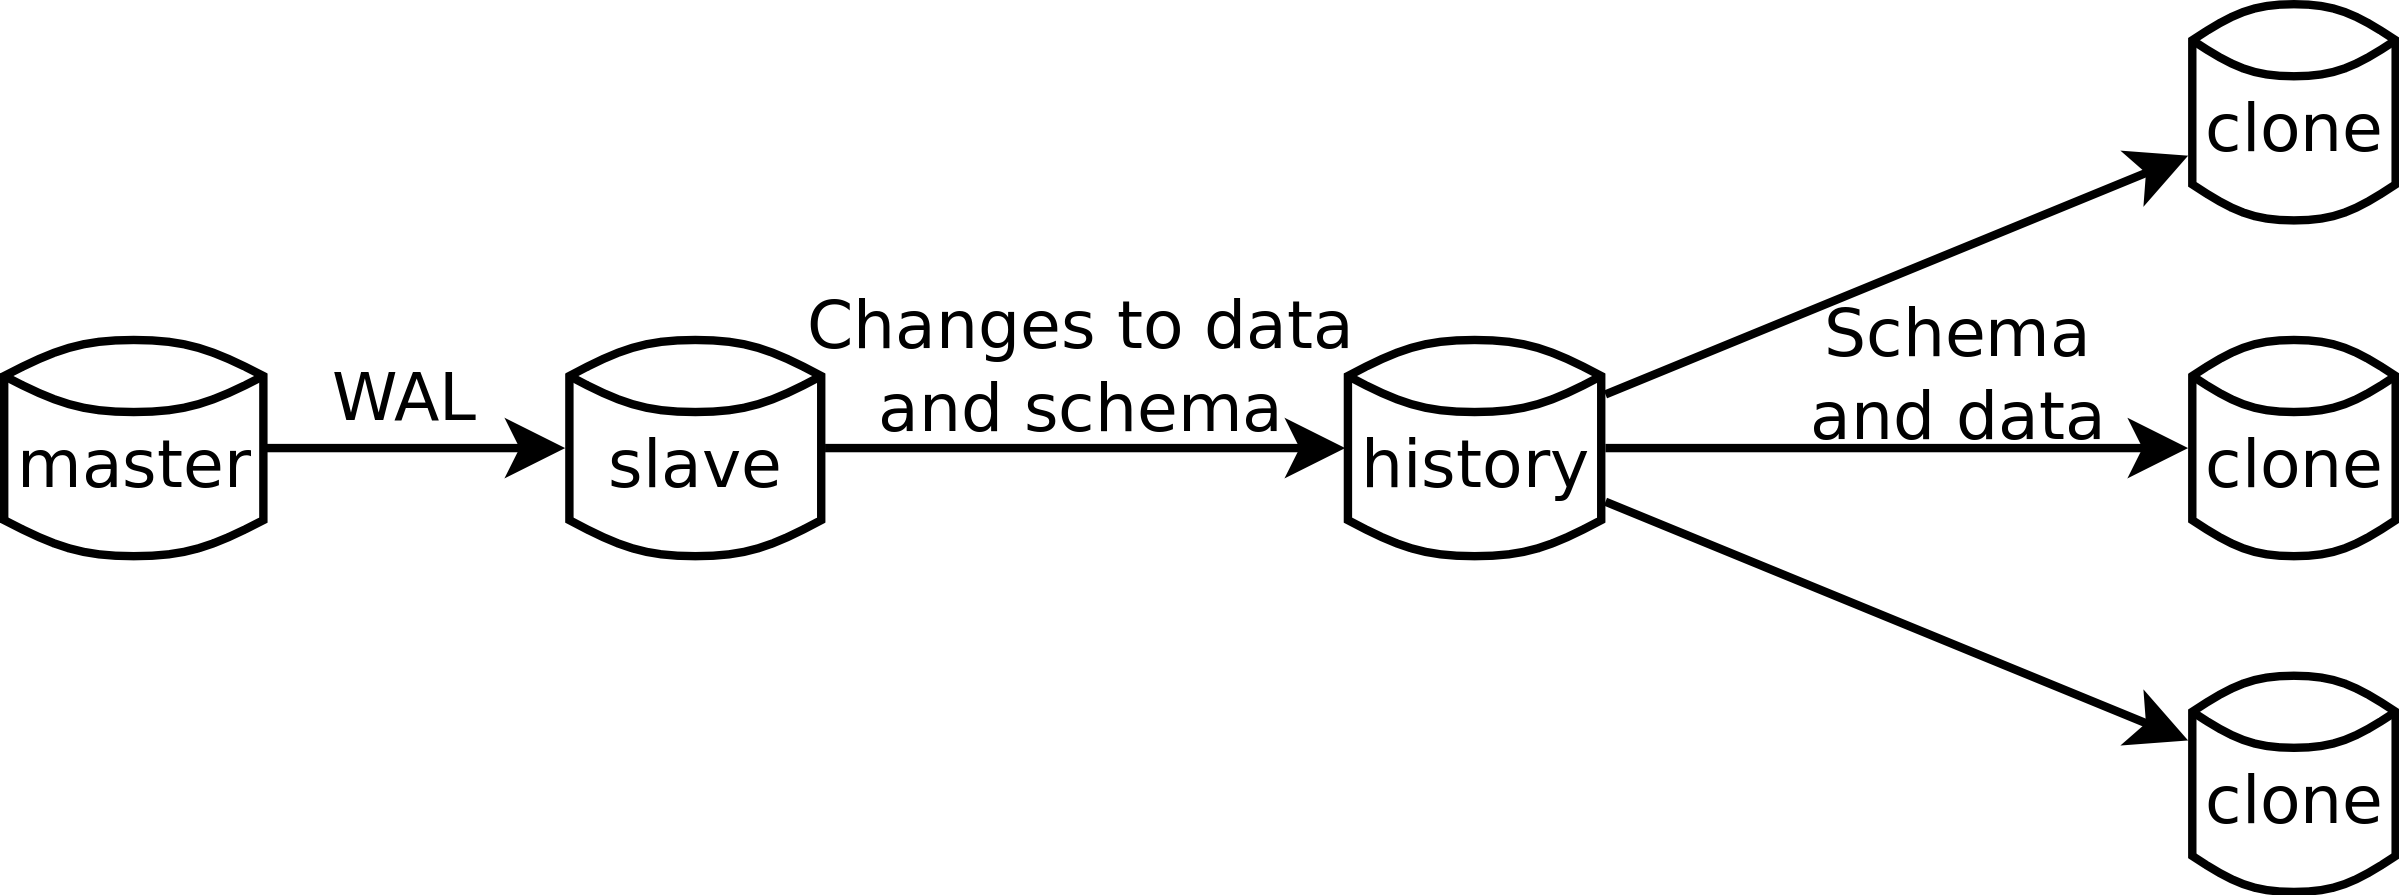
\includegraphics[width=0.8\textwidth]{architecture}
  \caption{An overview of the architecture of Marty}
  \label{architecture-overview}
\end{figure}

Marty does not inspect the schema of the master database directly when it creates the tabes in the clone databases.
Instead it queries another database that is called \textit{history}.
The history database contains information about the schema of the master database as well as a copy of its data.
When the clones need to populate their tables they also use this history database as a reference.
The reason for using another database to store a copy of the schema and data of the master database is discussed in chapter TODO, along with a description of the design of the history database.

As the name suggests the history database contains not only a copy of the current version of the master but also of previous versions.
To update the history database with new versions of the master and to keep it in sync with the changes that are made on the master Marty uses a log from the master that is called the \textit{write-ahead log} or \textit{WAL}.
It does not read this log directly but uses a specially patched instance of Postgres to read the contents of the log.
This instance is called \textit{slave} and it outputs information that Marty can use to update the history database with all the changes that have been made in the master database.
The reason for keeping old versions of the master database and the relationship between the master, slave and history databases is described in detail in chapter TODO.

\section{The clone databases}
\label{sec:clones}
A clone database is a standard Postgres database.
It uses two Postgres extensions; the \textit{PL/pgSQL} extension that enables users to create stored procedures, and the \textit{dblink} extension which enables users to query another database directly from the clone database without using any external scripts or programs.
The clone can run on a local instance of Postgres on the developers' or testers' computer as long as the history database is accessible from that computer.
More than one clone database can run in parallel on the same instance of Postgres so each user can use many clones at the same time.

To create a clone the user creates a new, empty database.
She then initializes it with Marty.
After the clone has been initialized it contains all the schemas that are found in the master database and a copy of all the tables from each schema.
The tables remain empty until they are first queried which saves time in the initialization as the user does not have to wait for Marty to finish copying all the data in the tables before she can start querying the clone.
This behaviour is implemented by creating views instead of tables in the clone.
The views look like the tables that the user expects to find and when they are queried they call a PL/pgSQL function, \textit{view\_select}, that returns the appropriate data.
This function looks for the data in the actual data tables, which Marty creates in the clone, and if these tables are empty the function populates them with data from the history database before returning their contents.

The data tables are created in a special schema called \textit{marty} which is created in the clone database.
It contains the data tables as well as another table called bookkeeping.
The view\_select function uses this table to keep track of which data tables have been populated and which ones are still unpopulated.
The table also contains the querystrings that view\_select uses when it fetches the data from the history database.
See figure \ref{clone-architecture} for an example of a table layout in a clone database.

The views, bookkeeping table, data tables and the view\_select function are described in detail in chapter TODO.

\begin{figure}[h!]
  \centering
    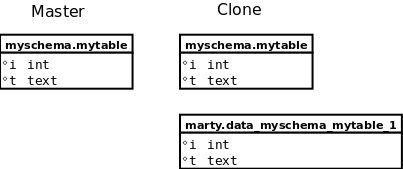
\includegraphics[width=0.5\textwidth]{clone-architecture}
  \caption{Table layout in a clone database}
  \medskip
  \small
  The table \textit{persons} is actually a view that returns results from the table \textit{data\_myschema\_persons\_1} which is in the \textit{marty} schema.
  \label{clone-architecture}
\end{figure}

\section{The history database}
The history database is a standard Postgres database.
It is created by a system administrator and contains data that the developers and testers use when they create clone databases.
When the history database has been initialized it contains information about the schema of the master database and a copy of its data.
After the initialization Marty updates the history database with all the changes that are made in the master, both to its data and schema.
Its contents are versioned and, as the name suggests, the user can look up previous states of the master in the history database.

The reason for keeping old versions of the master is the delayed population of the data tables in the clones.
From the moment that a clone database is initialized and until its tables are populated the master database might change.
Tables might be dropped or renamed and rows might be updated or deleted, which could lead to inconsistency in the clone as foreign key relations might break.
The history database offers access to a particular version of the contents of the master database and thus prevents errors of this kind in the clones.

Marty initializes the history database with four tables; \textit{marty\_schemas}, \textit{marty\_tables}, \textit{marty\_columns} and \textit{marty\_updates}.
The first three store information about the schemas, tables and table columns in the master database.
Their contents are mostly copied from the tables \textit{pg\_namespace}, \textit{pg\_class} and \textit{pg\_attributes}, respectively.
The fourth table, \textit{marty\_updates}, keeps a log of version timestamps.
Each version of the contents of the history database has two timestamps associated with it; the local time of the history server when that version was created in the history database and the time of the transaction on the master database that created that version.

Marty copies the data from the tables in the master and stores it in special data tables in the history database.
Each table in the master has a corresponding data table in the history database.
Its schema is similar to the original table but a few columns are added.
They are used for versioning and as a reference when rows are deleted or updated.
There are also no constraints on the data tables or their columns.
They are unnecessary as the data table is only used to store the data that has already been validated on the master.
Constraints might also get in the way, e.g. when the tables need to store different versions of the same row that has a unique constraint on some of its columns.
Another example might be a table that is altered and a not-null constraint is added to one of its columns where null values have been stored in the past.
Therefore there are no constraints on the data tables in the history database.
For an example of the schema of a data table see figure \ref{history-data-table}, and for further details see chapter TODO.

\begin{figure}[h!]
  \centering
    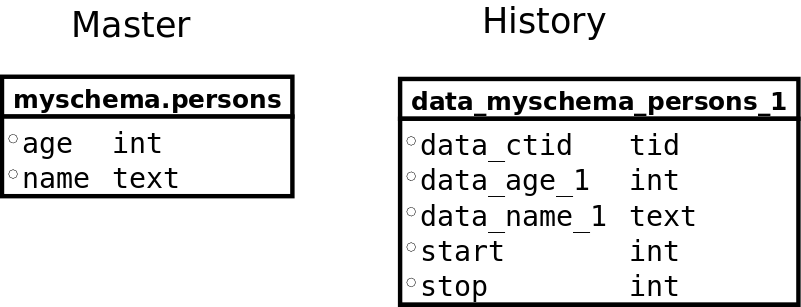
\includegraphics[width=0.5\textwidth]{history-data-table}
  \caption{An example of the schema of a data table in the history database}
  \label{history-data-table}
\end{figure}

\subsection{Populating and updating the history database}
When the history database is initialized its contents are not read directly from the master database.
Instead there is a dedicated instance of Postgres that replicates the master database that is used as a reference for the history.
This instance is called \textit{slave}.
The reason for using another instance to read the schema and data from the master is the format of the write-ahead log, or WAL.

The contents of the WAL are used to update the history database with the changes that are made to the master after the history has been initialized.
This approach was chosen because it makes it possible to read the changes that are made to the master database without inspecting it directy, e.g. with triggers.
That was considered important in the design process for Marty because any change on the master might introduce bugs and reduce its performance.
However, the WAL contains binary information and to be able to read it and use its contents it is necessary to have the database cluster files from the master as a reference.
Instead of implementing a complex algorithm to read the contents of the WAL it was decided to leverage on the recovery feature of Postgres that reads the WAL and applies it to the database cluster.
The slave is therefor started with a copy of the cluster files from the master database and it then replays the WAL into the cluster as it arrives from the master.
As it does so it logs all the operations that it replays and Marty uses this log to find and read the new version of the data from the slave.

The WAL debug log that logs all the operations is not enabled by default and the slave must therefor be compiled with special flags to enable it.
The replay must also be paused after each transaction that has been replayed to give Marty time to read the data from that transaction before the next one is applied.
To be able to do that it is necessary to patch Postgres and so the slave therefor runs on a specially patched version of Postgres.
More information about the slave can be found in chapter TODO.

\section{Advantages and Drawbacks}
The current architecture of Marty that is described in this chapter was chosen because of its simplicity and because it could be implemented in high level code (PL/pgSQL instead of C) which sped up prototyping and simplified the development of Marty.
However, it has a few drawbacks which make it unsuitable for a production ready version of Marty.
The main drawback is the lack of optimization for queries from the clones to the history database; when a user queries a table in a clone database it fetches the complete contents of that table from the history database even if the query should only return a small part of it to the user.
Another issue is the creation of indexes for the tables in the clones; the user can not create indexes for the tables in the clone like she would create them on the master database.
This is because the tables that the user expects to find in the clone database are actually views and it is not possible to create indexes for views in Postgres.

See chapter TODO for a discussion of the current status of Marty, the limitations of the current version and ideas for future works and improvements.
